\section{Linear classification}
\begin{itemize}
	\item Input $\bm{x}=\left(x_1, x_2, ..., x_D\right)^T$ with $\bm{x}\in\mathbb{R}^D$.
	\item Target $t\in\left\{C_1, C_2, ..., C_K\right\}$ with $K$ classes (one-hot representation)
	\item Goal: divide input space $\mathbb{R}^D$ into $K$ decision regions $R_k$ with $k=1,...,K$
	\item Boundaries of decision regions are called \textit{decision boundaries/surfaces}
	\begin{itemize}
		\item Linear classification only considers \textit{linear} decision boundaries $\Rightarrow$ $D-1$ dimensional hyperplanes
		\item A dataset is \textit{linearly separable}, if its classes can be exactly separated by linear decision boundaries
	\end{itemize}
	\item First, we derive the optimal solution for decision boundaries in general (3.1 Decision Theory), and then look at different models for deriving such solutions (3.2-3.4) 
\end{itemize}
\subsection{Decision Theory For Classification}
\begin{itemize}
	\item For every observed datapoint: label/ground truth $t_n=C_j$, prediction $t_n=C_k$
	\item Confusion matrix (row: GT class, columns: prediction region/class)
	$$\begin{blockarray}{ccccc}
	& R_1 & R_2 & \dots & R_K \\
	\begin{block}{c(cccc)}
	C_1 & 6 & 1 & \dots & 0 \\
	C_2 & 4 & 2 & \dots & 3 \\
	\vdots & \vdots & \vdots & \ddots & \vdots \\
	C_K & 1 & 0 & \dots & 5 \\
	\end{block}
	\end{blockarray}$$
	\begin{itemize}
		\item The elements on the diagonal represent the correctly classified examples
		\item Try to minimize misclassified examples (off-diagonal elements), or the probability of a mistake: $p\left(\text{mistake}\right) = 1 - \sum\limits_{k=1}^{K}p(\bm{x}\in R_k, C_k)$
	\end{itemize}
	\item Assign $x$ to class $C_k$ if $\forall j\neq k: p\left(\bm{x}, t=C_k\right) > p\left(\bm{x}, t=C_j\right)$ $\Rightarrow$ $p\left(C_k|\bm{x}\right) > p\left(C_j|\bm{x}\right)$
	\item Optimal decision boundary where $p\left(C_k|\bm{x}\right) = p\left(C_j|\bm{x}\right)$
	\item Problem: \textit{class imbalance} $\Rightarrow$ possible solution: weighted loss for balancing the importance of each class
	\item For imbalanced datasets, assign $x$ to $C_k$ if $\sum\limits_{j=1}^{K}L_{jk}p\left(x,C_j\right)$ is minimal 
	\begin{itemize}
		\item $L_{jk}$ is misclassification weight matrix where $L_{ii}=0$
		\item Example for dataset with 1\% cancer patients: 
		$$L = \begin{blockarray}{ccc}
		\text{pred. cancer} & \text{pred. healthy} & \\
		\begin{block}{(cc)c}
		0 & 1000 & \text{true cancer} \\
		1 & 0 & \text{true healthy} \\
		\end{block}
		\end{blockarray}$$
	\end{itemize}
\end{itemize}
\subsection{Probabilistic generative models}
\begin{itemize}
	\item Model the class conditional densities $p\left(x|C_k\right)$ \textbf{and} the prior class probabilities $p(C_k)$ to compute posterior probabilities $p\left(C_k|x\right)$ (as we know from Decision Theory that at $p\left(C_k|x\right)=p\left(C_j|x\right)$ are the optimal decision boundaries)
	\item For $K=2$, the posterior is: $p\left(C_1|\bm{x}\right) = \frac{p\left(\bm{x}|C_1\right)p\left(C_1\right)}{p\left(\bm{x}\right)} = \frac{p\left(\bm{x}|C_1\right)p\left(C_1\right)}{p\left(\bm{x}|C_1\right)p\left(C_1\right) + p\left(\bm{x}|C_2\right)p\left(C_2\right)}$
	\item We can simplify the previous equation by using the sigmoid function:
	\begin{equation*}
		\begin{split}
			p\left(C_1|\bm{x}\right) & = \frac{1}{1 + \frac{p\left(\bm{x}|C_2\right)p\left(C_2\right)}{p\left(\bm{x}|C_1\right)p\left(C_1\right)} } = \frac{1}{1+\exp\left(-a\right)} \text{\hspace{5mm}where\hspace{5mm}} a=\ln\frac{\sigma}{1-\sigma} = \ln \frac{p\left(\bm{x}|C_2\right)p\left(C_2\right)}{p\left(\bm{x}|C_1\right)p\left(C_1\right)}
		\end{split}
	\end{equation*}
	\item For general $K$: $p\left(C_k|\bm{x}\right) = \frac{p\left(\bm{x}|C_k\right)p\left(C_k\right)}{\sum_{j=1}^{K}p\left(\bm{x}|C_j\right)p\left(C_j\right)} = \frac{\exp(a_k)}{\sum_{j=1}^{K} \exp(a_j)}$ with $a_k = \ln \left[ p\left(\bm{x}|C_k\right)p\left(C_k\right)\right]$ (softmax)
	\item In the special case of $K=2$: $a=a_1-a_2$
\end{itemize}
\subsubsection{Continuous inputs}
\begin{itemize}
	\item Assume that the class-conditional  densities are Gaussian:
	$$p\left(\bm{x}|C_k\right) = \mathcal{N}\left(\bm{x}|\bm{\mu}_k,\bm{\Sigma}_k\right) = \frac{1}{\left(2\pi\right)^{D/2}}\frac{1}{|\bm{\Sigma}_k|^{1/2}}\exp\left\{\frac{1}{2}\left(\bm{x}-\bm{\mu}_k\right)^T\bm{\Sigma}^{-1}\left(\bm{x}-\bm{\mu}_k\right)\right\}$$
	\item We assume that all classes share the same covariance: $\bm{\Sigma}_k = \bm{\Sigma}$\\$\Rightarrow$ We are able to apply \textbf{linear discriminant analysis} (otherwise, decision boundaries would be quadratic)
	\item Determining posterior for $K=2$:
	\begin{equation*}
		\begin{split}
			a & = \ln \frac{p\left(\bm{x}|C_2\right)p\left(C_2\right)}{p\left(\bm{x}|C_1\right)p\left(C_1\right)} = \ln \mathcal{N}\left(\bm{x}|\bm{\mu}_1,\bm{\Sigma}_1\right) - \ln \mathcal{N}\left(\bm{x}|\bm{\mu}_2,\bm{\Sigma}_2\right) + \ln \frac{p\left(C_1\right)}{p\left(C_2\right)}\\
			& = \left(\bm{\mu}_1 - \bm{\mu}_2\right)^T\bm{\Sigma}^{-1}\bm{x} - \frac{1}{2}\bm{\mu}_1^T\bm{\Sigma}^{-1}\bm{\mu}_1 + \frac{1}{2}\bm{\mu}_2^T\bm{\Sigma}^{-1}\bm{\mu}_2 + \ln \frac{p\left(C_1\right)}{p\left(C_2\right)}
		\end{split}
	\end{equation*}
	\item Thus, the posterior can be expressed by
	\begin{equation*}
		\begin{split}
			p(C_1|\bm{x})=\sigma\left(\bm{w}^Tx+w_0\right) \text{\hspace{3mm}where\hspace{2mm}} & \bm{w} = \bm{\Sigma}^{-1}\left(\bm{\mu}_1 - \bm{\mu}_2\right)\\
			& w_0 = -\frac{1}{2}\bm{\mu}_1^T\bm{\Sigma}^{-1}\bm{\mu}_1 + \frac{1}{2}\bm{\mu}_2^T\bm{\Sigma}^{-1}\bm{\mu}_2 + \ln \frac{p\left(C_1\right)}{p\left(C_2\right)}
		\end{split}
	\end{equation*} 
	\item For general $K$, we get $p\left(C_k|\bm{x}\right) = \frac{\exp\left(a_k\left(\bm{x}\right)\right)}{\sum_{j=1}^{K}\exp\left(a_j\left(\bm{x}\right)\right)}$ with 
	\begin{equation*}
	\begin{split}
	a_k\left(\bm{x}\right) = \ln \left[p\left(\bm{x}|C_k\right)\cdot p\left(C_k\right)\right]=\bm{w}_k^Tx+w_{k0} \text{\hspace{3mm}where\hspace{2mm}} & \bm{w}_k = \bm{\Sigma}^{-1}\bm{\mu}_k\\
	& w_{k0} = -\frac{1}{2}\bm{\mu}_k^T\bm{\Sigma}^{-1}\bm{\mu}_k + \ln p\left(C_k\right)
	\end{split}
	\end{equation*} 
	\item Decision boundaries are at $p\left(C_k|\bm{x}\right) = p\left(C_j|\bm{x}\right)$ $\Rightarrow$ $a_k = a_j\Rightarrow$ Linear decision boundaries!
	\begin{figure}[ht]
		\centering
		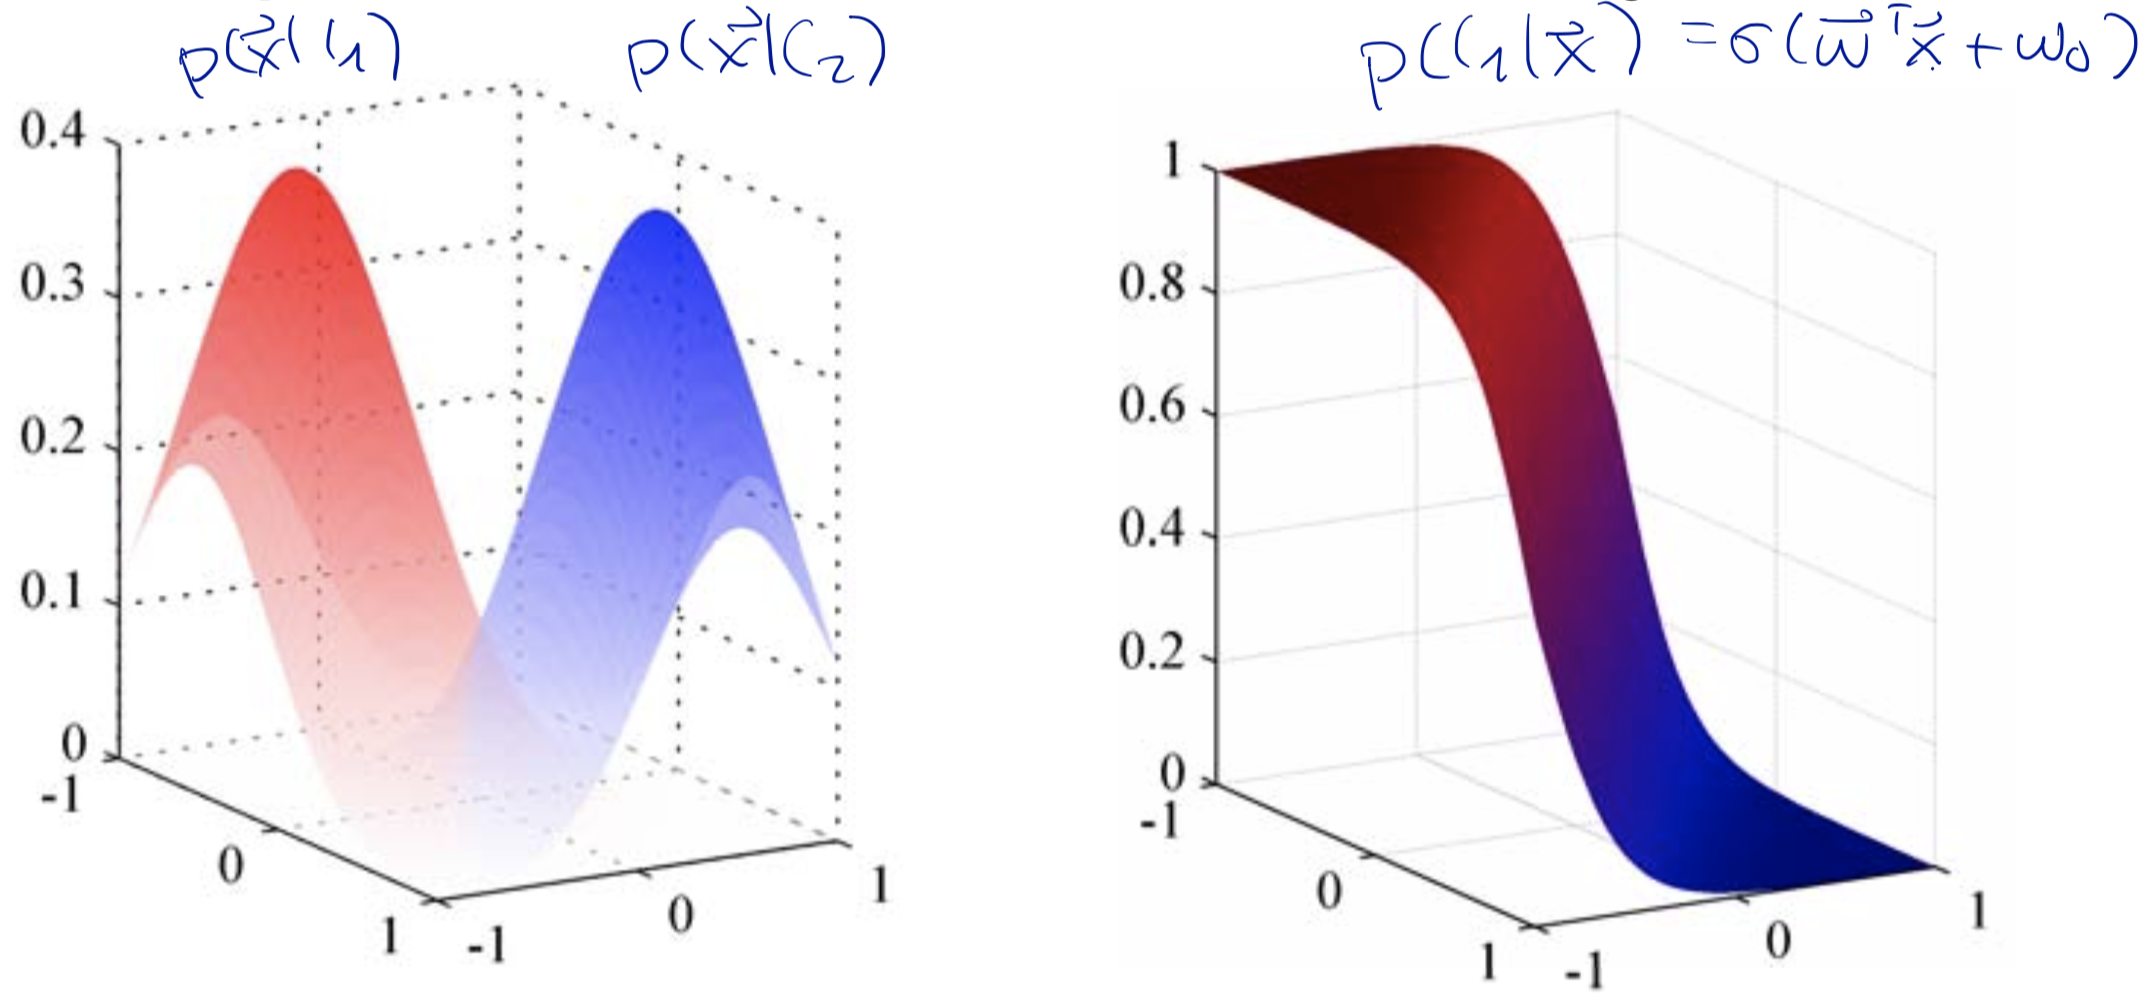
\includegraphics[width=0.7\textwidth]{figures/linear_classification_pgm.png}
		\caption{Left: Gaussian class-conditional densities, Right: corresponding posterior with sigmoid}
	\end{figure}
\end{itemize}
\subsubsection{Maximum likelihood solution for $K=2$}
\begin{itemize}
	\item Binary targets $t_n\in\left\{0,1\right\}$ ($1$ for $C_1$, $0$ for $C_0$)
	\item We use maximum likelihood to find optimal solution for $\bm{\mu}_k$, $\bm{\Sigma}$ and priors $p\left(C_k\right)$
	\item For $K=2$, the priors are denoted by $p\left(C_1\right) = q$ and $p\left(C_2\right) = 1-q$
	\item If $\bm{x}_n$ has target $t_n=1$: $p\left(\bm{x}_n, C_1\right) = p\left(\bm{x}_n|C_1\right)p\left(C_1\right) =q\mathcal{N}\left(\bm{x}_n|\bm{\mu}_1, \bm{\Sigma}\right)$
	\item If $\bm{x}_n$ has target $t_n=0$: $p\left(\bm{x}_n, C_2\right) = p\left(\bm{x}_n|C_2\right)p\left(C_2\right) =(1-q)\mathcal{N}\left(\bm{x}_n|\bm{\mu}_2, \bm{\Sigma}\right)$
	\item Combined likelihood: $p\left(\bm{t}, \bm{X}|q,\bm{\mu}_1,\bm{\mu}_2,\bm{\Sigma}\right) = \prod\limits_{n=1}^{N} \left[q\mathcal{N}\left(\bm{x}_n|\bm{\mu}_1, \bm{\Sigma}\right)\right]^{t_n}\left[(1-q)\mathcal{N}\left(\bm{x}_n|\bm{\mu}_2, \bm{\Sigma}\right)\right]^{1-t_n}$
	\item Log-likelihood: $$\ln p\left(\bm{t}, \bm{X}|q,\bm{\mu}_1,\bm{\mu}_2,\bm{\Sigma}\right) = \sum\limits_{n=1}^{N}t_n \ln q + t_n \ln \mathcal{N}\left(\bm{x}_n|\bm{\mu}_1, \bm{\Sigma}\right) + (1 - t_n) \ln \left(1 - q\right) + \left(1 - t_n\right) \ln \mathcal{N}\left(\bm{x}_n|\bm{\mu}_2, \bm{\Sigma}\right) $$
	\item Estimate for $q$: $\frac{\partial}{\partial q} \ln p\left(\bm{t}, \bm{X}|q,\bm{\mu}_1,\bm{\mu}_2,\bm{\Sigma}\right) = \sum\limits_{n=1}^{N} \frac{t_n}{q} - \frac{1 - t_n}{1 - q} = \sum\limits_{n=1}^{N} \frac{t_n - q}{q\left(1 - q\right)} \Rightarrow q_{\text{ML}} = \frac{1}{N}\sum\limits_{n=1}^{N} t_n = \frac{N_1}{N}$\\
	- Thus, the estimate of $p(C_1)$ is the proportion of samples that are assigned to class 1
	\item Estimate for $\bm{\mu_1}$: $\bm{\mu}_{1,\text{ML}} = \frac{1}{N_1}\sum\limits_{n=1}^{N} t_n \bm{x}_n$, $\bm{\mu}_{2,\text{ML}} = \frac{1}{N_2}\sum\limits_{n=1}^{N} \left(1-t_n\right) \bm{x}_n$\\
	- Thus, the estimate of $\bm{\mu}_k$ is the mean of the samples assigned to class $k$
	\item Estimate for $\bm{\Sigma}$: 
	$$\bm{\Sigma}_{\text{ML}} = \frac{N_1}{N}\underbrace{\left[\frac{1}{N_1} \sum\limits_{n=1}^{N} t_n\left(\bm{x} - \bm{\mu}_{1,\text{ML}}\right)\left(\bm{x} - \bm{\mu}_{1,\text{ML}}\right)^T\right]}_{\text{sample covariance of class 1}} + \frac{N_2}{N}\underbrace{\left[\frac{1}{N_2} \sum\limits_{n=1}^{N} (1-t_n)\left(\bm{x} - \bm{\mu}_{2,\text{ML}}\right)\left(\bm{x} - \bm{\mu}_{2,\text{ML}}\right)^T\right]}_{\text{sample covariance of class 2}}$$
	- Thus, the estimate of $\bm{\Sigma}$ is a weighted average (based on number of samples for each class) of the class' sample covariance\\
	- Note that this assumes a similar covariance matrix for every class cluster. If this is not the case, the estimation gives bad results (see Figure~\ref{img:linear_discriminative_analysis_different_cov})
	\begin{figure}[ht]
		\centering
		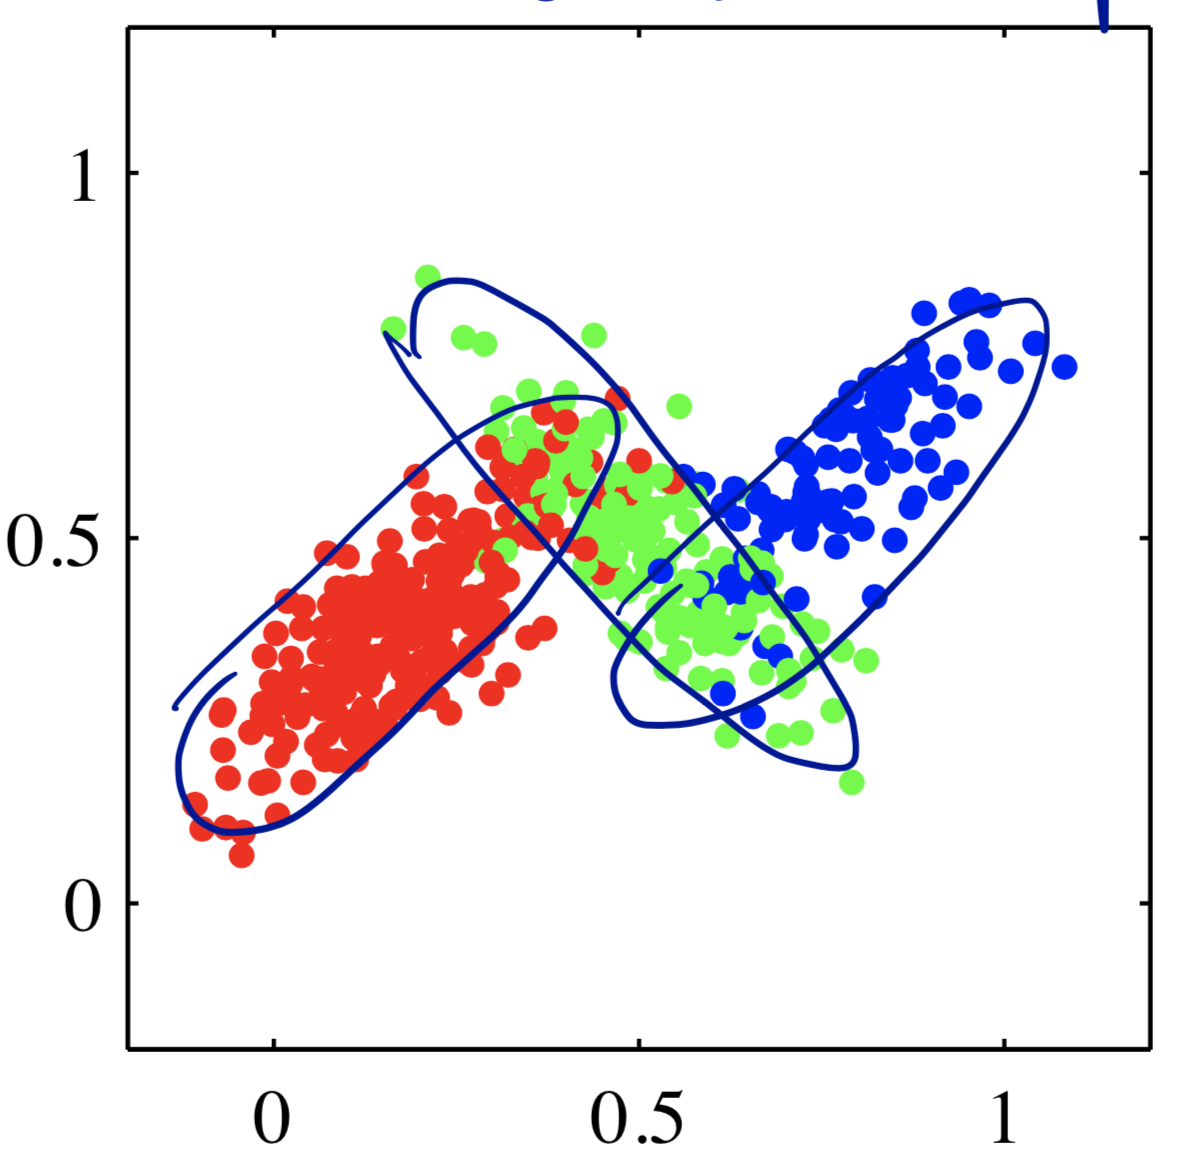
\includegraphics[width=0.2\textwidth]{figures/linear_discriminant_analysis_different_cov.png}
		\caption{Example for three classes with different covariance matrices $\bm{\Sigma}_k^{-1}$. Linear discriminant analysis fails as it estimates a weighted sum of the sample covariance, and the distribution of green class significantly differs from the other two. The resulting estimate would tend to be a circle for each class instead of the drawn ellipses.}
		\label{img:linear_discriminative_analysis_different_cov}
	\end{figure}
\end{itemize}
\subsubsection{Discrete inputs}
\begin{itemize}
	\item In contrast to the previous subsections, we now assume that $\bm{x}_n \in\left\{0,1\right\}^D$ and is therefore discrete
	\item As we know have no PDF anymore, we need $2^D - 1$ parameters per class to guarantee a perfect fit
	\item However, if we use the Naive Bayes assumption (feature values are treated as independent given $C_k$), we reduce the number of features to $D$ per class (by using the Bernoulli distribution):
	$$p\left(\bm{x}|C_k\right) = \prod\limits_{i=1}^{D}p\left(x_i|C_k\right) = \prod\limits_{i=1}^{D} \pi_{ki}^{x_i}\left(1 - \pi_{ki}\right)^{1-x_i}$$
	\item We can apply this simplification to rewrite $a_k$:
	$$a_k = \ln p\left(x|C_k\right) + \ln p\left(C_k\right)  = \sum\limits_{i=1}^{D}\left[x_i\ln \pi_{ki} + (1 - x_i)\ln (1 - \pi_{ki}) \right] + \ln p\left(C_k\right) = \bm{x}^T\bm{w} + w_0 $$
	 where $w_i=\ln \frac{\pi_{ki}}{1 - \pi_{ki}}$ and $w_0 = \ln p\left(C_k\right) + \sum_{i=1}^{D}\ln \left(1-\pi_{ki}\right)$ 
\end{itemize}
\subsection{Discriminant functions}
\begin{itemize}
	\item Direct mapping of input to target (similar to regression)%$t=y(x,w)$
	\item We use $y\left(\bm{x},\bm{\tilde{w}}\right) = f\left(\bm{\tilde{w}}^T\bm{\phi}\right)$, where $f$ is the activation function and might be non-linear 
	\item The decision boundary is defined at a point where $y\left(\bm{x},\bm{\tilde{w}}\right) = \text{const}_1$. As $y$ represents the application of $f$, we can rewrite it as $\bm{\tilde{w}}^T\bm{\phi} = \text{const}_2$
	\item We first review the application of the case of two classes, and then try to find a solution for multiple classes
\end{itemize}
\subsubsection{Discriminant functions for two classes}
\begin{itemize}
	\item For a two class problem, we set the decision boundary to 0 as we are still able to shift it by $w_0$
	\item If $y\left(\bm{x},\bm{\tilde{w}}\right)\geq 0$, the input $\bm{x}$ is assigned to class $C_1$, whereas if $y\left(\bm{x},\bm{\tilde{w}}\right)< 0$, the class is $C_2$ $\Rightarrow w_0$ is considered as the activation threshold
	\item To determine how the weights $\bm{\tilde{w}}$ influence this classification, we assume two points $\bm{x}_a$ and $\bm{x}_b$ on the decision boundary $\Rightarrow$ $y\left(\bm{x}_a\right) = y\left(\bm{x}_b\right) = 0 \Rightarrow \bm{w}^T(\bm{x}_a - \bm{x}_b) = 0$ (see Figure~\ref{img:discriminant_function_two_classes})
	\item Hence, $\bm{w}$ is orthogonal to every vector lying within the decision surface, so that $\bm{w}$ determines the orientation of the surface
	\begin{figure}[ht]
		\centering
		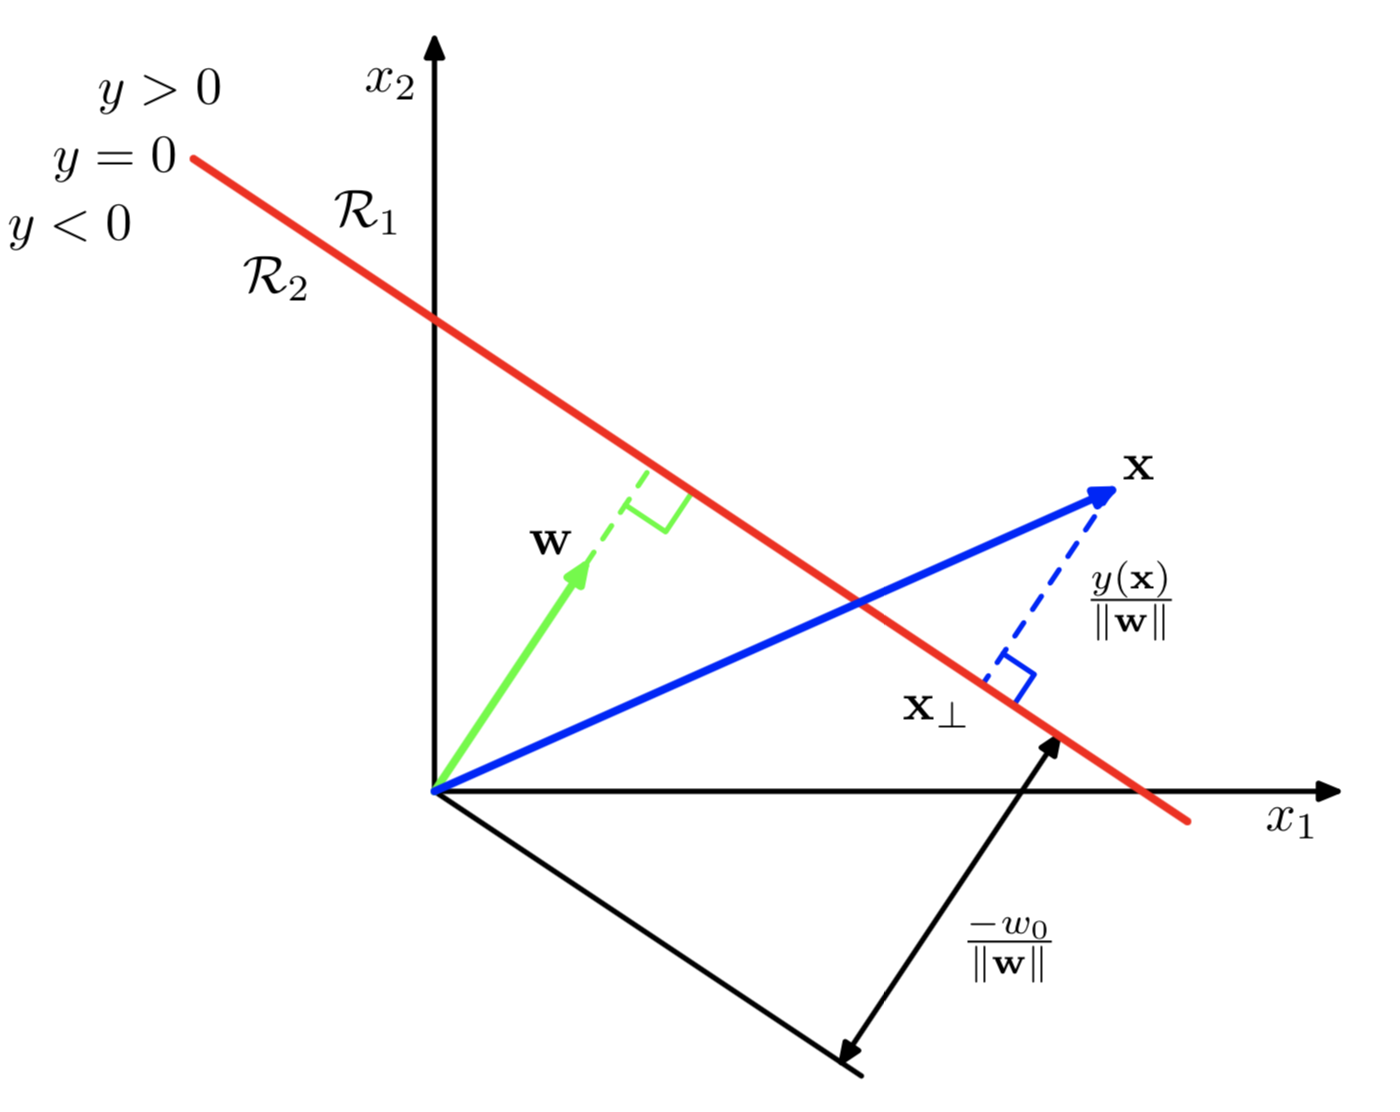
\includegraphics[width=0.4\textwidth]{figures/discriminant_function_two_classes.png}
		\caption{Illustration of the geometry of a linear discriminant function in two dimensions. The decision surface, shown in red, is perpendicular to $\bm{w}$, and its displacement from the origin is controlled by the bias parameter $w_0$. Also, the signed orthogonal distance of a general point $\bm{x}$ from the decision surface is given by $y(\bm{x})/ \bm{w}$ .}
		\label{img:discriminant_function_two_classes}
	\end{figure}
	\item So, we can express every point by the summation of a point on the decision surface and the weights: $$\bm{x} = \bm{x}_{\perp} + r\frac{\bm{w}}{||\bm{w}||}$$
	\item Applied in $y$, we get: $y\left(\bm{x}\right) = \bm{w}^T \bm{x} + w_0 = \bm{w}^T \bm{x}_{\perp} + w_0 + r\frac{\bm{w}^T\bm{w}}{||\bm{w}||} = r ||\bm{w}|| \Rightarrow $
	\item So, the distance between a point $\bm{x}$ and the decision surface is $r = \frac{y\left(\bm{x}\right)}{||\bm{w}||}$
\end{itemize}
\subsubsection{Discriminant functions for multiple classes}
\begin{itemize}
	\item K-class discriminant: $\bm{y}_k (\bm{x}) = \bm{w}_k^T + w_{k0}$
	\item Assign $\bm{x}$ to $C_k$ if $y_k(\bm{x})>y_j(\bm{x})$ for all $j\neq k$
	\item Thus, the decision boundary between $\mathcal{R}_k$ and $\mathcal{R}_j$ is determined by: $y_k(\bm{x})=y_j(\bm{x})$
	\item Note that decision regions of linear discriminant functions are convex (if two points are in $\mathcal{R}_k$, then all points between those are also in the same region $\mathcal{R}_k$)
\end{itemize}
\subsubsection{Least squares discriminant}
\begin{itemize}
	\item Consider $\bm{t}_n$ as one-hot vector. We try to learn a function $y_k(\bm{x}, \bm{\tilde{w}}_k)$ for every class $k$ that maps $\bm{x}$ to its corresponding value in the one-hot vector (basically regression task)
	\item For shorter notation, we write $\bm{y}(\bm{x}) = \bm{\tilde{W}}\bm{\tilde{x}}$ to combine all classes and weights into a single operation
	\item As before: assign $\bm{x}$ to class $C_k$ if $k=\arg\max_j y_j (\bm{x})$
	\item The error function is the sum-of-squares: $$E_D(\bm{\tilde{W}}) = \frac{1}{2} \text{Tr}\left[\left(\bm{\tilde{X}}\bm{\tilde{W}}-\bm{T}\right)^T\left(\bm{\tilde{X}}\bm{\tilde{W}}-\bm{T}\right)\right] = \frac{1}{2}\sum\limits_{n=1}^{N}\sum\limits_{k=1}^{K}\sum\limits_{d=1}^{D}\left(\tilde{X}_{nd}\tilde{W}_{dk}-\tilde{T}_{nd}\right)$$
	\item Minimizing this error leads to:  $\bm{\tilde{W}}_{\text{LS}} = \left(\bm{\tilde{X}}^T \bm{\tilde{X}}\right)^{-1}\bm{\tilde{X}}^T \bm{\tilde{T}}$
	\item But: there are many problems with least squared errors
	\begin{itemize}
		\item The decision boundaries are very sensitive to outliers (try to minimizes \textit{mean} error to one-hot vector)
		\item For $K>2$, some decision regions become very small or are even completely ignored (also called masking)
		\item components of $\bm{y}_{\text{LS}}$ are not probabilities and can be outside the interval $\left[0,1\right]$
	\end{itemize}
	\begin{figure}[ht]
		\centering
		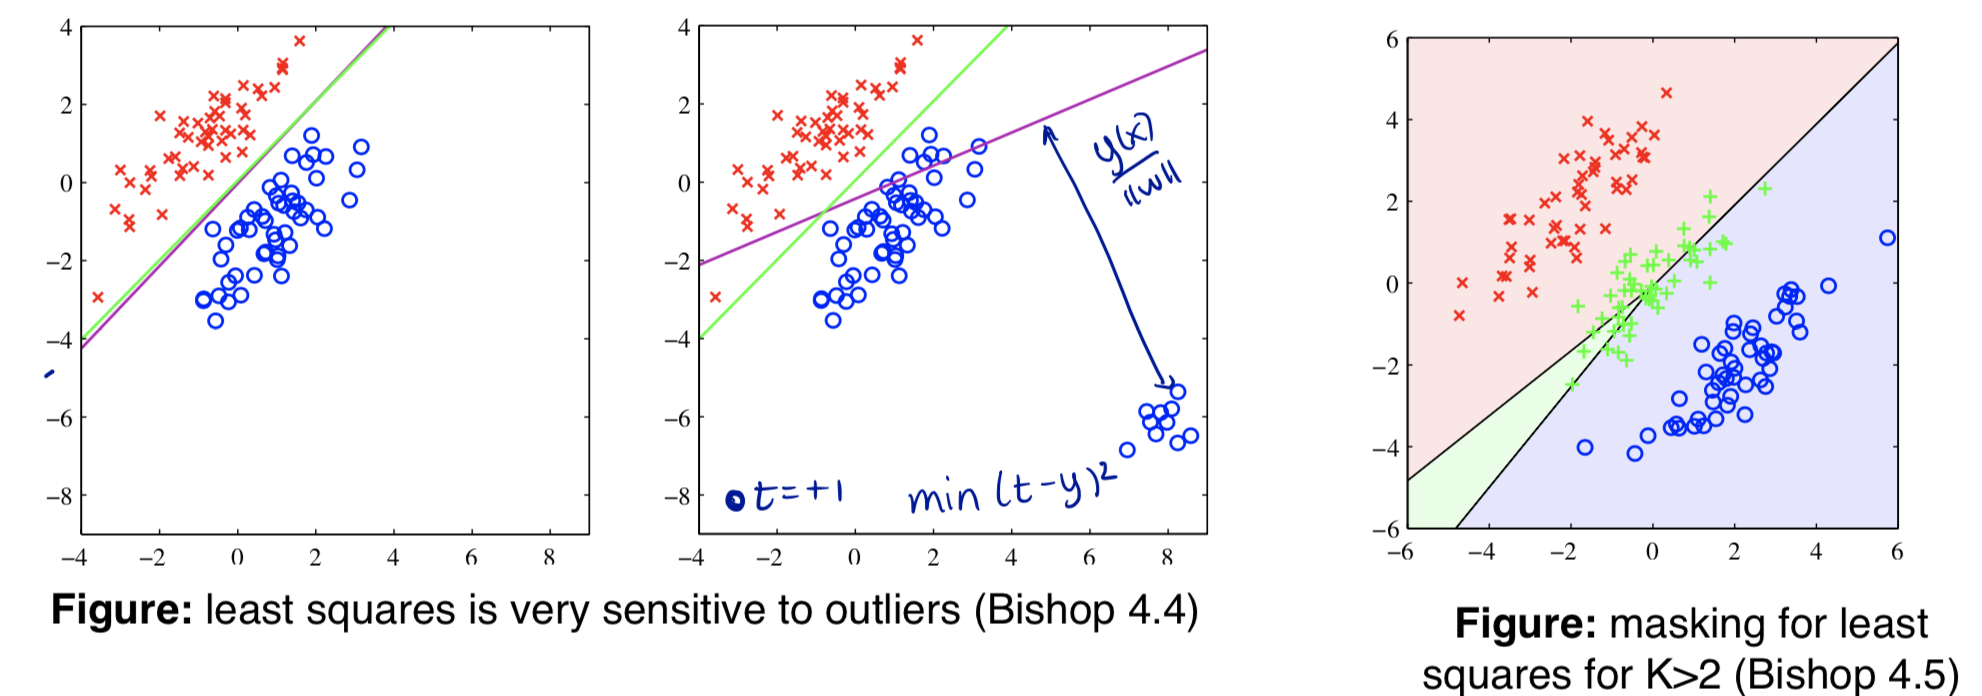
\includegraphics[width=0.6\textwidth]{figures/discriminant_function_least_squares_problem.png}
		\caption{Illustration of the problems with least squared error discriminant}
		\label{img:discriminant_function_least_squares_problem}
	\end{figure}
\end{itemize}
\subsubsection{Perceptron}
\begin{itemize}
	\item For the perceptron, we use the step function as activation function:
	$$y\left(\bm{x}\right) = f\left(\bm{w}^T\bm{\phi}(\bm{x})\right) \text{\hspace{5mm} where \hspace{5mm}} f(a) = \begin{cases}
	1 & \text{ if } a\geq 0\\
	-1 & \text{ if } a <0
	\end{cases}$$
	\item Thus, assign $\bm{x}$ to class $C_1$ if $\bm{w}^T\bm{\phi}(\bm{x})\geq0$, otherwise $C_2$
	\item The goal is now to find a $\bm{w}$ such that $\bm{w}^T\bm{\phi}(\bm{x})t_n\geq 0$ ($t_n \in \left\{1,-1\right\}$)
	\item We can define the error of a perceptron based on the set of misclassified examples $\mathcal{M}$: \\$E_P(\bm{w})=-\sum\limits_{n\in\mathcal{M}}\bm{w}^T \bm{\phi}(\bm{x}_n)t_n = \sum\limits_{n\in\mathcal{M}}E_n(\bm{w})$
	\item Use Stochastic Gradient Descent (SGD) for each misclassified $\bm{x}_n$:\\ $$\bm{w}^{\tau+1} = \bm{w}^{\tau} - \eta \bigtriangledown^T E_n(\bm{w}) = \bm{w}^{\tau} + \eta \bm{\phi}(\bm{x}_n) t_n$$
	\item If $\bm{X}$ is linearly separable, SGD will converge
	\item However, there are some problems with the perceptron algorithm:
	\begin{itemize}
		\item Perceptron only works for 2 classes
		\item There might be many optimal solutions, so that the exact outcome depends on initialization of $\bm{w}$ and order of data that are used in SGD
		\item If dataset is not linearly separable, the perceptron algorithm will not converge
		\item Based on linear combination of fixed basis functions 
	\end{itemize}
\end{itemize}
\subsubsection{Usage of Basis functions}
\begin{itemize}
	\item If the data in the input space is not linearly separable, we can use basis functions (that might be non-linear) to transform them into a new space, where they can be linearly separated!
	\item However, prior knowledge is required for this step as the general data distribution must be known and how to convert it into a linearly separable space. This step is especially hard/not possible for high dimensions
\end{itemize}
\subsection{Probabilistic discriminative models}
\begin{itemize}
	\item Instead of specifying the class-conditional probabilities $p\left(\bm{x}|C_k\right)$ and applying maximum likelihood to find the best parameters, we can try to explicitly model the posterior class probability $p\left(C_k|\bm{x}\right)$ and find its distribution $\Rightarrow$ posteriors are non-linear functions with a linear function of $\bm{\phi}$ as input: $p\left(C_k|\bm{\phi}, \bm{w}\right) = f(\bm{w}_k^T\bm{\phi})$
	\item The implicit method of finding the parameters of a generalized model is by fitting $p\left(\bm{x}|C_k\right)$ and $p\left(C_k\right)$ representing a generative model (generate synthetic data from $p(\bm{x})$)
\end{itemize}
\subsubsection{Logistic regression for two classes}
\begin{itemize}
	\item Logistic regression uses the sigmoid function to model the posterior:\\
	$$p\left(C_1|\bm{\phi},\bm{w}\right) = y\left(\bm{\phi}\right) = \sigma\left(\bm{w}^T\bm{\phi}\right), p\left(C_2|\bm{\phi},\bm{w}\right) = 1 - p\left(C_1|\bm{\phi},\bm{w}\right)$$
	\item For inference/classification, take the class with the higher probability ($>0.5$) $\Rightarrow$ Decision boundaries: $\bm{w}\bm{\phi}(\bm{x}) = 0$
	\item If $\bm{w}\in\mathbb{R}^M$, we use $M$ number of parameters (compared to $M(M+5)/2 + 1$ for modeling a Gaussian multivariate distribution)
	\item Use maximum likelihood to determine the parameters of the logistic regression model
	\item Conditional likelihood: $p\left(\bm{t}|\bm{X},\bm{w}\right) = \prod\limits_{n=1}^{N} p\left(t_n | \bm{x}_n,\bm{w}\right) = \prod\limits_{n=1}^{N} y_n^{t_n}\left(1 - y_n\right)^{1-t_n}$
	\item Maximizing the likelihood is equal to minimizing the cross-entropy loss:
	$$E(\bm{w}) = -\ln p\left(\bm{t}|\bm{X},\bm{w}\right) = -\sum\limits_{n=1}^{N} \left[t_n \ln y_n + (1 - t_n) \ln (1 - y_n)\right] =\sum\limits_{n=1}^{N}E_n(\bm{w})$$
	\item The loss $E(\bm{w})$ is convex (has a single, \textbf{unique minimum}), but no closed-form solution exists ($y_n = \sigma(\bm{w}^T \phi_n)$ is nonlinear in $\bm{w}$) $\Rightarrow$ Use SGD/...
	\item For taking the gradient, we can make use of the property of the sigmoid function: 
	$$\frac{\partial E_n(\bm{w})}{\partial w_j} = \frac{\partial E_n(\bm{w})}{\partial y_n} \frac{\partial y_n}{\partial w_j} = \left[-\frac{t_n}{y_n}+\frac{1 - t_n}{1 - y_n}\right] \cdot \left[\sigma(\bm{w}^T\bm{\phi}(\bm{x}_n))\left(1 - \sigma(\bm{w}^T\bm{\phi}(\bm{x}_n))\right) \phi_j(\bm{x}_n)\right] = (y_n - t_n)\phi_j(\bm{x}_n)$$
	\item Update rule (SGD): $\bm{w}^{\tau + 1} = \bm{w}^{\tau} - \eta \triangledown^{\tau} E_n(\bm{w})^{\tau}= \bm{w}^{\tau} - \eta (y_n - t_n)\bm{\phi}\left(\bm{x}_n\right)$
	\item If $\eta$ too large: no convergence. If $\eta$ too small: very slow convergence
	\item Converged $\bm{w}^*$ minimizes the loss $E(\bm{w})$
\end{itemize}
\subsubsection{Iterative reweighted least squares}
\begin{itemize}
	\item Also called the \textit{Newton-Raphson iterative optimization scheme}
	\item We use a \textbf{quadratic approximation} instead of a linear at $E(\bm{w}^{\tau})$ as the difference between the difference of the loss function to a second order polynomial is quite small (find $E(\bm{w}^{\tau+1})$ that minimizes our quadratic approximation $\Rightarrow$ no learning rate)
	\item New update rule: $$\bm{w}^{\tau} = \bm{w}^{\tau-1} - \bm{H}^{-1} \triangledown E(\bm{w}^{\tau - 1})$$ where $\bm{H}$ is the Hessian matrix whose elements comprise the second derivatives of $E(\bm{w})$: $H_{ij}=\frac{\partial E(\bm{w})}{\partial w_i \partial w_j}$ ($\bm{H}$ is symmetric!)
	\item Derived from the previous section, the gradient for all $N$ data-points is 
	$$\triangledown E(\bm{w}) = \sum\limits_{n=1}^{N} (y_n - t_n)\bm{\phi}\left(\bm{x}_n\right) = \bm{\Phi}^T\left(\bm{y} - \bm{t}\right)$$
	\item The elements of the Hessian derive this by a second parameter again:
	$$H_{ij} = \frac{\partial E(\bm{w})}{\partial w_i \partial w_j} = \frac{\partial}{\partial w_i}\sum\limits_{n=1}^{N} (y_n - t_n)\phi_j \left(\bm{x}_n\right) = \sum\limits_{n=1}^{N} \phi_j\left(\bm{x}_n\right) \frac{\partial y_n}{\partial w_i} = \sum\limits_{n=1}^{N} y_n (1 - y_n) \phi_i(\bm{x}_n)\phi_j(\bm{x}_n)$$
	\item The overall Hessian matrix is therefore 
	$$\bm{H} = \sum\limits_{n=1}^{N} y_n (1 - y_n) \bm{\phi}(\bm{x}_n)\bm{\phi}(\bm{x}_n)^T = \bm{\Phi}^T \bm{R}\bm{\Phi}$$
	where $R_{nn} = y_n(1-y_n)$, and otherwise $R_{nm} = 0$ for $n\neq m$
	\item Applying this term in the update equation leads to:
	$$\bm{w}^{(\tau)} = \bm{w}^{(\tau - 1)} - \left(\bm{\Phi}^T \bm{R} \bm{\Phi}\right)^{-1}\bm{\Phi}^T\left(\bm{y} - \bm{t}\right) = \left(\bm{\Phi}^T \bm{R} \bm{\Phi}\right)^{-1} \bm{\Phi}^T \bm{z} \text{\hspace{5mm}where\hspace{5mm}} \bm{z} = \bm{\Phi}\bm{w}^{(\tau-1)}-\bm{R}^{-1}(\bm{y}-\bm{t})$$
	\item Note the similarity to the maximum likelihood solution $\bm{w}_{\text{ML}} = \left(\bm{\Phi}^T \bm{\Phi}\right)^{-1} \bm{\Phi}^T\bm{t}$
	\begin{figure}[ht]
		\centering
		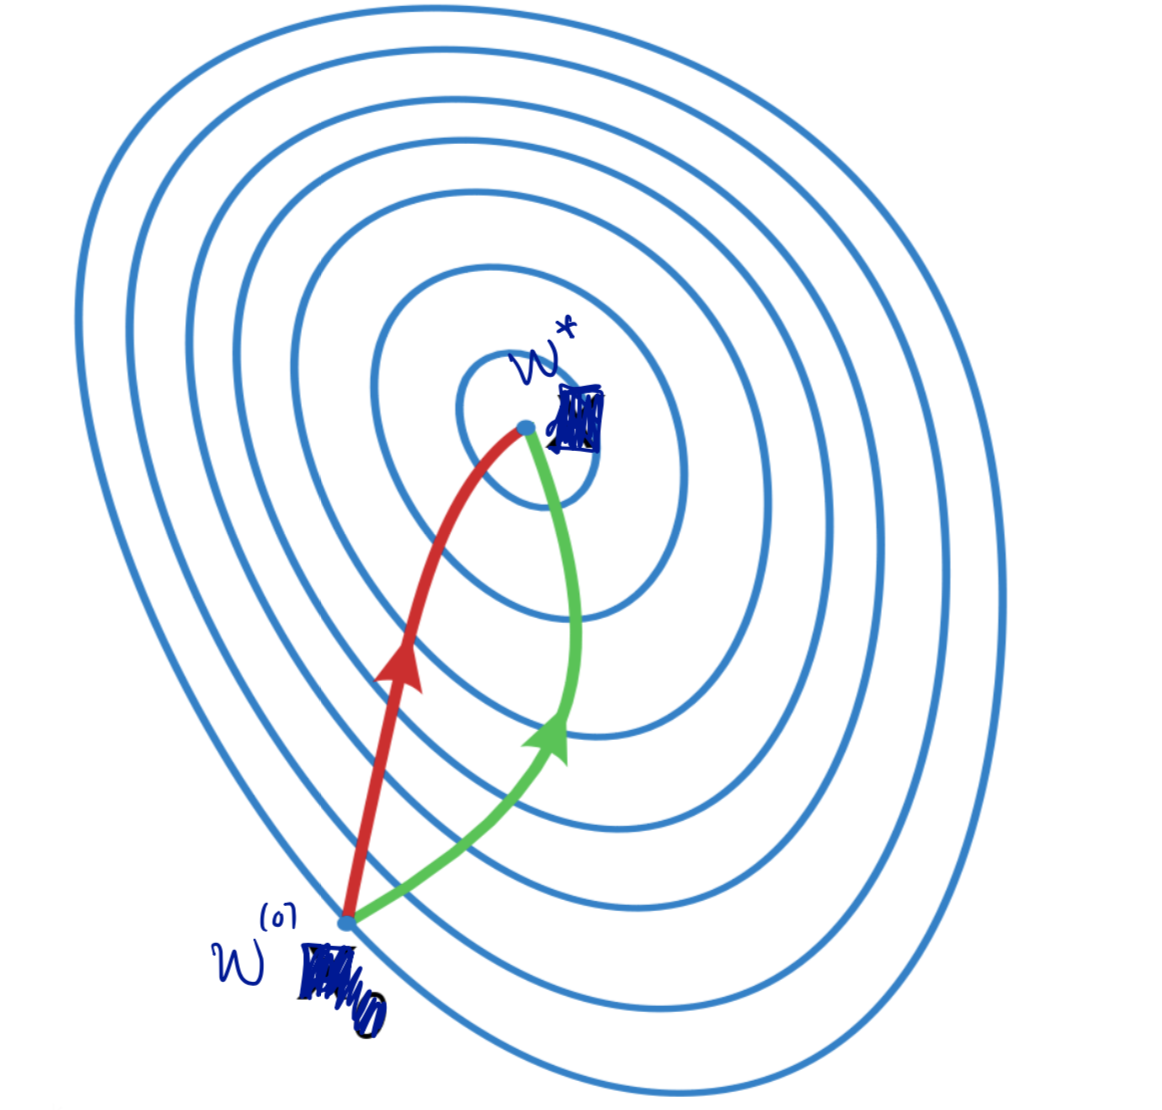
\includegraphics[width=0.4\textwidth]{figures/logistic_regression_sgd_iterat.png}
		\caption{Illustration of SGD (green) and Newton Raphson (red). SGD always goes in the direction of the steepest gradient and is therefore slower than Newton-Raphson.}
		\label{img:logistic_regression_sgd_iterat}
	\end{figure}
\end{itemize}
\subsubsection{Logistic regression for multiple classes}
\begin{itemize}
	\item Our posterior distribution is now given by a softmax:
	$$p(C_k|\bm{\phi}, \bm{w}_1, ..., \bm{w}_K) = y_k\left(\bm{\phi}\right) = \frac{\exp\left(a_k\right)}{\sum_{j=1}^{K}\exp\left(a_j\right)} \text{\hspace{5mm}where\hspace{5mm}} a_k=\bm{w}_k^T\bm{\phi}(\bm{x})$$
	\item The derivation by a element $a_j$ is $\frac{\partial y_k}{\partial a_j}=y_k\left(\mathbb{I}\left(k=j\right) - y_j\right)$
	\item We use again maximum likelihood to determine the optimal parameters
	\item Conditional likelihood $p\left(\bm{T}|\bm{X},\bm{w}_1,...\bm{w}_K\right) = \prod\limits_{n=1}^{N}\prod\limits_{k=1}^{K}p(C_k|x_k, \bm{w}_1, ..., \bm{w}_K) = \prod\limits_{n=1}^{N}\prod\limits_{k=1}^{K} y_{k}\left(\bm{\phi}_n\right)^{t_{nk}}$
	\item Taking the negative logarithm gives the \textit{cross-entropy} loss function for the multiclass classification problem
	$$E\left(\bm{w}_1,...,\bm{w}_K\right) = - \ln p\left(\bm{T}|\bm{w}_1,...,\bm{w}_K\right) = -\sum\limits_{n=1}^{N}\sum\limits_{k=1}^{K} t_{nk} \ln y_{nk}$$
	\item To minimize the function by SGD or Newton Raphson, we need to take the derivate:
	$$\triangledown_{\bm{w}_j} E\left(\bm{w}_1, ...,\bm{w}_K\right) = \sum\limits_{n=1}^{N}\left(y_{nj} - t_{nj}\right) \bm{\phi}\left(\bm{x}_n\right)$$
	\item For Newton Raphson/Iterative reweighted least squares, we also need the Hessian matrix:
	$$\frac{\partial}{\partial \bm{w}_k}\frac{\partial}{\partial \bm{w}_j}E\left(\bm{w}_1,...,\bm{w}_K\right) = \sum\limits_{n=1}^{N} y_{nk}\left(\mathbb{I}\left(k=j\right) - y_{nj}\right) \bm{\phi}_n \bm{\phi}_n^T$$
	\item Decision boundaries at $\left(\bm{w}_k^*\right)^T \bm{\phi}\left(\bm{x}'\right) = \left(\bm{w}_j^*\right)^T \bm{\phi}\left(\bm{x}'\right)$
\end{itemize}